\section{Sliding Mode}
Now, with the system on \textit{regular form}, the sliding mode controller can be designed.
The sliding manifold is chosen:
\begin{flalign}
  s &=   \xi - \phi(\vec{\eta}) = 0     \ \ \ , &
\end{flalign}
where $\phi(\vec{\eta})$ must be designed. When the system is restricted to move along $s = 0$ then $\xi = \phi(\vec{\eta})$, which means the reduced-order model,
\begin{flalign}
  \vec{\dot{\eta}} &=  f_a(\vec{\eta},\phi(\vec{\eta}))     \ \ \ , &
  \label{eq:asymStabOrigReducedOrder}
\end{flalign}
is asymptotically stable in its origin. To find a stabilizing controller, $\phi(\vec{\eta})$, for \autoref{eq:asymStabOrigReducedOrder}, the reduced-order system is linearized,
%
\begin{flalign}
  A &= \frac{\partial \vec{\dot{\eta}}}{\partial \vec{\eta}} \whereThree{\vec{\eta}=\vec{0}\ \ \ \ }{\xi=0\ \ \ \ }{\text{k}_\text{tanh}=1} \ 
  =
  \begin{bmatrix}
    0 & -1                  & 0 \\
    0 & \frac{g_{p,c}}{l m} & g \\
    0 & 0                   & 0 
  \end{bmatrix}   \ \ \ , \ \ \
  B = \frac{\partial \vec{\dot{\eta}}}{\partial \xi} \whereThree{\vec{\eta}=\vec{0}\ \ \ \ }{\xi=0\ \ \ \ }{\text{k}_\text{tanh}=1} \ 
  =
  \begin{bmatrix}
    l  \\
    \frac{-b_{p,v}-b_{p,c}}{l m}  \\
    1  
  \end{bmatrix}   \ \ \ , & 
  \label{eq:linearReducedOrder_A}
\end{flalign}
%
Using the matlab \textit{place()} command, different pole-placements were attempted, seen in \autoref{fig:reducedOrderControlMany}. The chosen pole placement is $[\ -3\ \ -5\ \ -8\ ]$ resulting in the state feedback gains, $\vec{k} = [\ -12.22\ \ 8.05\ \ 20.10\ ]$, of which the result is seen in \autoref{fig:reducedOrderControl}, where the linear simulation is achieved using \textit{lsim()} and the nonlinear using \textit{ode45}. \fxnote{fix formatting on matlab function reff.'s}
\begin{adjustwidth}{-1.2cm}{-1.2cm}
\begin{minipage}{\textwidth}
  \begin{minipage}{0.58\textwidth}
    \begin{figure}[H]
      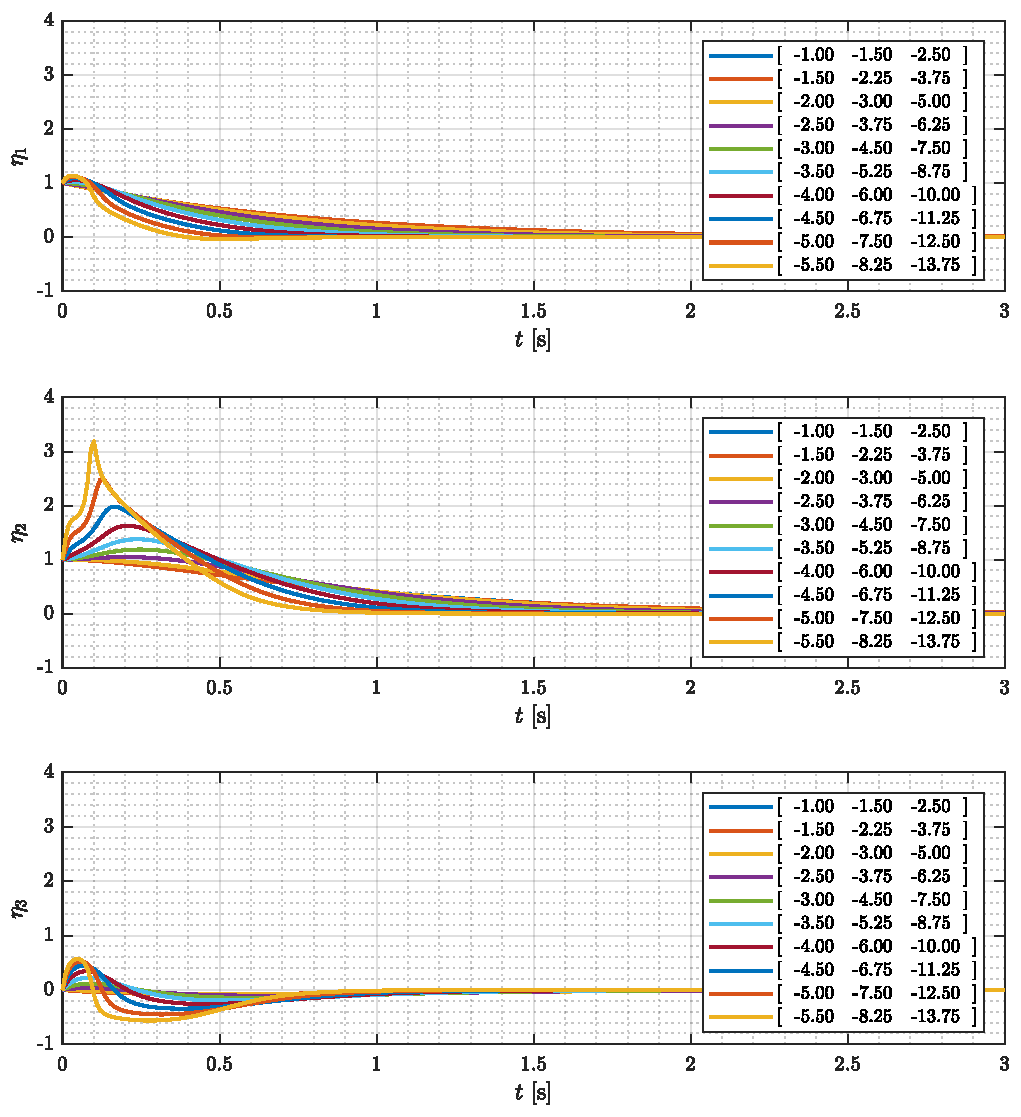
\includegraphics[width=\textwidth]{figures/reducedOrderControlMany}
      \caption{reducedOrderControlMany}
      \label{fig:reducedOrderControlMany}
    \end{figure}
  \end{minipage}
  \begin{minipage}{0.58\textwidth}
    \begin{figure}[H]
      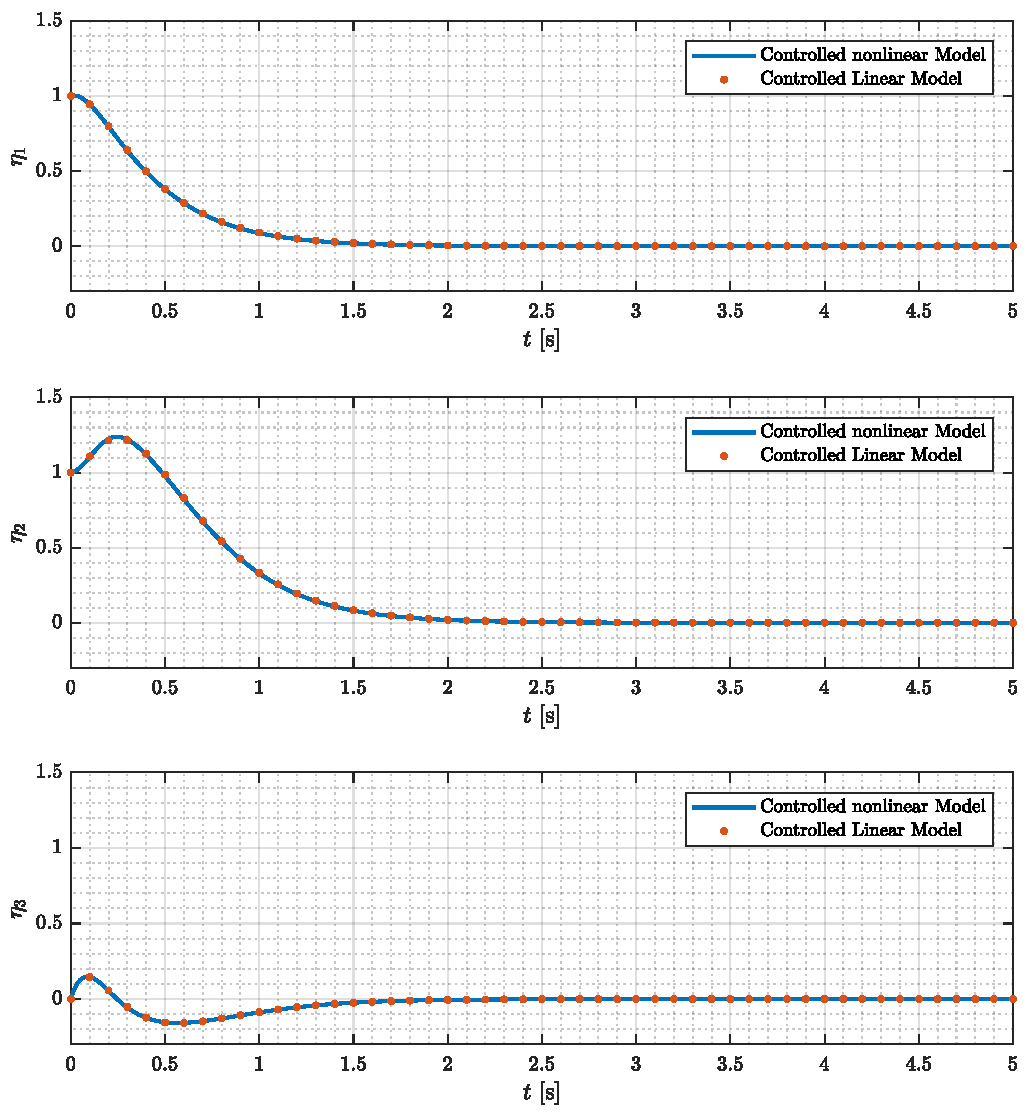
\includegraphics[width=\textwidth]{figures/reducedOrderControl}
      \caption{reducedOrderControl}
      \label{fig:reducedOrderControl}
    \end{figure}
  \end{minipage}
\end{minipage}
\end{adjustwidth}
With the reduced-order system stabilized by,
\begin{flalign}
  \phi(\vec{\eta}) &=   - \vec{k} \vec{\eta}  \ \ \ , &
\end{flalign}
next step is to design F to bring $s$ to zero.\\
First a Lyapunov function candidate, $V = \frac{1}{2}s^2$, is chosen and its derivative along the system's trajectories is found,
\begin{flalign}
  \dot{V} &= s\dot{s} & \\
  \dot{V} &= s ( \dot{\xi} + \vec{k}\vec{\dot{\eta}}  ) & \\
  \dot{V} &= s ( f_b(\vec{\eta},\xi) + g_b(\vec{\eta},\xi) F +\vec{k}f_a(\vec{\eta},\xi) )  & \\
  \dot{V} &= ( \vec{k}f_a(\vec{\eta},\xi)  +  f_b(\vec{\eta},\xi) )s + g_b(\vec{\eta},\xi) s F  & \\
  \dot{V} &= g_b(\vec{\eta},\xi) s (\vec{k}f_a(\vec{\eta},\xi)  +  f_b(\vec{\eta},\xi)) g_b^{-1}(\vec{\eta},\xi) + g_b(\vec{\eta},\xi) s F  &  \\
  \dot{V} &\leq g_b(\vec{\eta},\xi) |s| \left|\vec{k}f_a(\vec{\eta},\xi) g_b^{-1}(\vec{\eta},\xi) +  f_b(\vec{\eta},\xi) \right| + g_b(\vec{\eta},\xi) s F  \ \ \ . &
  \label{eq:lyapunov}
\end{flalign}
Using that $|s| = \text{sgn}(s) s$ to design $F$ such that the two terms in \autoref{eq:lyapunov} cancels and the stability criterion is fulfilled,
\begin{flalign}
\dot{V} &\leq g_b(\vec{\eta},\xi) |s| \left|\vec{k}f_a(\vec{\eta},\xi) +  f_b(\vec{\eta},\xi) \right|  g_b^{-1}(\vec{\eta},\xi)  & \nonumber \\
&- g_b(\vec{\eta},\xi) \text{sgn}(s) s \left|\vec{k}f_a(\vec{\eta},\xi)  +  f_b(\vec{\eta},\xi) \right| g_b^{-1}(\vec{\eta},\xi)  &
\label{eq:lyapunov2}
\end{flalign}
s.t.
\begin{flalign}
F &= -\text{sgn}(s)\varrho(\vec{\eta},\xi) g_b^{-1}(\vec{\eta},\xi) \ \ \ \ \text{where}, \ \ \ \varrho(\vec{\eta},\xi)  \geq \left|\vec{k}f_a(\vec{\eta},\xi)  +  f_b(\vec{\eta},\xi) \right|   \ \ \ , &
\label{eq:ssControlBeta}
\end{flalign}
further, a tuning parameter, $\beta_0$, is introduced,
\begin{flalign}
F &= -\text{sgn}(s)\beta (\vec{\eta},\xi) \ \ \ \ \text{where}, \ \ \ \beta(\vec{\eta},\xi) = \varrho(\vec{\eta},\xi) + \beta_0  \ \ \ . &
\label{eq:ssControlBeta0}
\end{flalign}
%where $\varrho(\vec{\eta},\xi)$ is redefined as an upper bound on $\left|\frac{\vec{k}f_a(\vec{\eta},\xi)  +  f_b(\vec{\eta},\xi)}{g_b(\vec{\eta},\xi)} \right|$ within the region of interest.\\
The gain design is based on a maximum possible catch angle, $\theta_\mathrm{max}$, which is defined from zero angular velocity. The position and velocity along $x$ does not interfere with the value of $\theta_\mathrm{max}$, so long as the angular velocity of the pendulum is zero. Note, if the pendulum is falling away from equilibrium, its non-zero angular velocity will work against the controller and the catch angle will be smaller. However, similarly, if the pendulum is approaching equilibrium, the controller's catch angle will be larger.\\
While there will be other combinations of $\theta$ and $\dot{\theta}$ in the region of interest requiring as much actuation as $(\theta,\dot{\theta})=(\theta_\mathrm{max},0)$, these initial values are chosen to be on the edge of the region in the proceeding design.\\
In \autoref{fig:chooseRho}, $\varrho(\vec{\eta},\xi)$ and the required peak armature current magnitude, $|i_{a,\mathrm{peak}}|$, are plotted for different initial angles, $\theta\mathrm{init}$, to see how large a gain is feasible while staying within the actuation limitation of the motor, $i_{a,\mathrm{max}} = \SI{4.58}{A}$, see \textit{Motors} \autoref{sec:motors}.
%
\begin{figure}[H]
  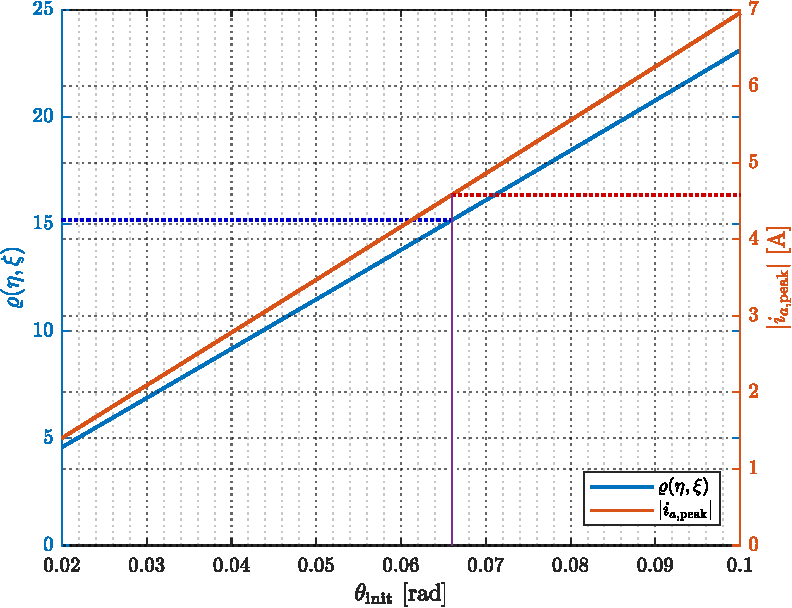
\includegraphics[width=.75\textwidth]{figures/chooseRho}
  \caption{$\dot{\theta}=0$ horizontal line marks $\theta_\mathrm{max} = 0.0660$ dictated by the current limitation of the motor, $i_{a,\mathrm{max}} = \SI{4.58}{A}$, and thereby indicating the maximum gain, $\varrho(\vec{\eta},\xi) = 15.1776$, with $\beta_0=0.1$, allowing some margin for the supposed operational region.}
  \label{fig:chooseRho}
\end{figure}




